\chapter{Speech processing}


\section{Audio representation}

\begin{description}
    \item[Sound/soundwave] \marginnote{Soundwave}
        Vibration that travels though a medium. It is modulated by:
        \begin{descriptionlist}
            \item[Pitch] Frequency of the vibrations.
            \item[Loudness] Amplitude of the vibrations. 
        \end{descriptionlist}

    \item[Waveform] \marginnote{Waveform}
        Representation of a soundwave. It is described by:
        \begin{description}
            \item[Frequency] 
                Represents the pitch of the sound.

            \item[Period] 
                Distance between two peaks of the sound (i.e., correlated to frequency as $f=\frac{1}{T}$).

            \item[Amplitude] 
                Represents the loudness of the sound (i.e., the air pressure).

                \begin{remark}
                    In practice, amplitude is usually converted in decibels due to the fact that the human auditory system perceives sound closer to a logarithmic scale.
                \end{remark}
        \end{description}

        \begin{figure}[H]
            \centering
            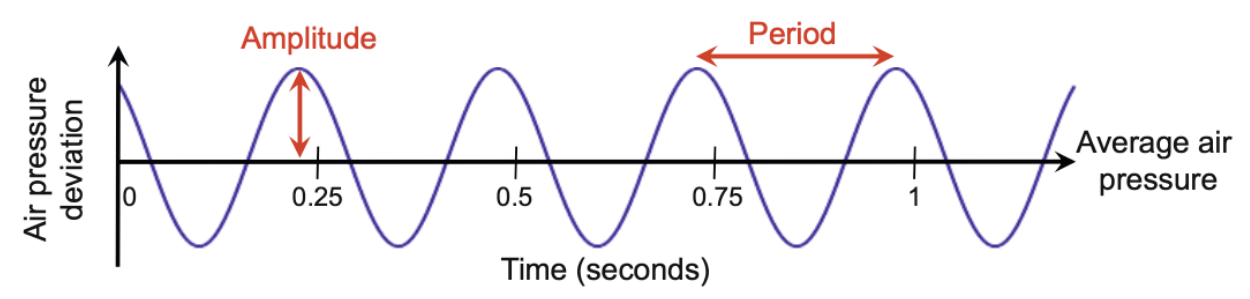
\includegraphics[width=0.7\linewidth]{./img/waveform.png}
        \end{figure}

    \item[Signal] \marginnote{Signal}
        Representation of information.

        \begin{remark}
            In sound processing, the waveform itself is the signal.
        \end{remark}

        \begin{description}
            \item[Analog signal] \marginnote{Analog signal}
                Waveform as-is in the real world.

            \item[Digital signal] \marginnote{Digital signal}
                Sampled (i.e., measure uniform time steps) and quantized (i.e., discretize values) version of an analog waveform.
        \end{description}

    \item[Fourier transform] \marginnote{Fourier transform}
        Method to decompose a continuous signal in its constituent sin waves.

        Given a continuous signal $x(t)$, its Fourier transform is:
        \[ X(f) = \int_{-\infty}^{+\infty} x(t) e^{-j2\pi ft} \,dt \]
        where $X(f)$ indicates how much of the frequency $f$ exists in $x(t)$.

        \begin{description}
            \item[Discrete Fourier transform (DFT)] \marginnote{Discrete Fourier transform (DFT)}
                Fourier transform for digital signals.

                Given a discrete signal $x[n]$, its DFT is:
                \[ X[k] = \sum_{n=0}^{N-1} x[n]e^{-\frac{j2\pi kn}{N}} \]
                where $k$ is the discrete frequency and $N$ is the number of samples.

            \item[Fast Fourier transform (FFT)] \marginnote{Fast Fourier transform (FFT)}
                Efficient implementation of DFT for $N$s that are power of $2$.

            \item[Short-time Fourier transform (STFT)] \marginnote{Short-time Fourier transform (STFT)}
                FFT computed on short time windows of the sound signal.

                \begin{remark}
                    This method allows preserving time information by using a fixed frame size.
                \end{remark}

                \begin{description}
                    \item[Spectrogram] \marginnote{Spectrogram}
                        Result of STFT that shows how the frequencies change over time.
                \end{description}

                \begin{figure}[H]
                    \centering
                    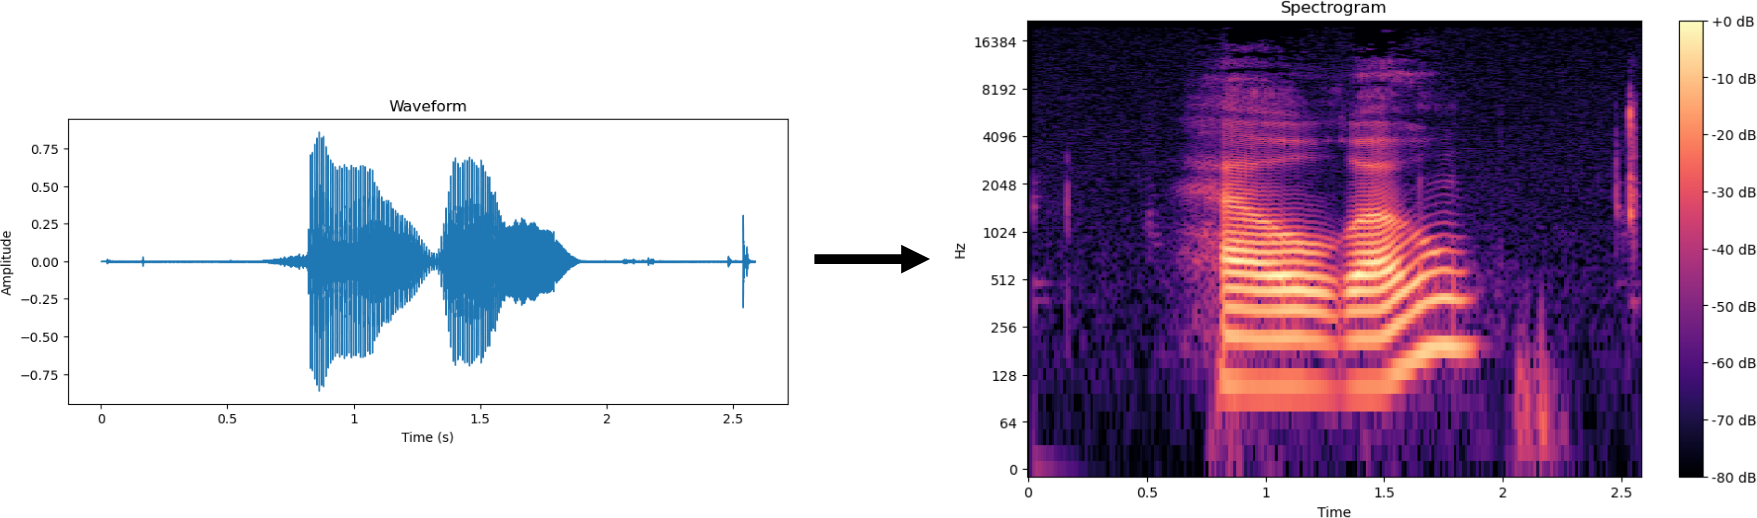
\includegraphics[width=0.8\linewidth]{./img/spectrogram.png}
                \end{figure}

            \item[Inverse STFT (ISTFT)] \marginnote{Inverse STFT (ISTFT)}
                Converts a time-frequency representation of sound (i.e., spectrogram) to its sound signal.

                \begin{remark}
                    This allows to manipulate a signal in its frequency domain (STFT) and then convert it back (ISTFT).
                \end{remark}
        \end{description}

    \item[Mel-scaled spectrogram] \marginnote{Mel-scaled spectrogram}
        Spectrogram where frequencies are mapped to the mel scale (i.e., lower frequencies are more fine-grained while higher frequencies are more compressed, to match the human logarithmic sound perception).

    \item[Audio features] \marginnote{Audio features}
        Representation of a sound signal extracted from the waveform or spectrogram.
\end{description}



\section{Tasks}

\begin{description}
    \item[Automatic speech recognition (ASR)]
        Convert a sound signal into text.

        \begin{example}
            Use an RNN/transformer encoder-decoder architecture. A sound signal is processed as follows:
            \begin{enumerate}
                \item Compute the audio features from the waveform (e.g., mel-spectrogram).
                \item Pass the computed features through the encoder.
                \item Use the decoder to generate the output text autoregressively conditioned on the encoder.
            \end{enumerate}

            \begin{figure}[H]
                \centering
                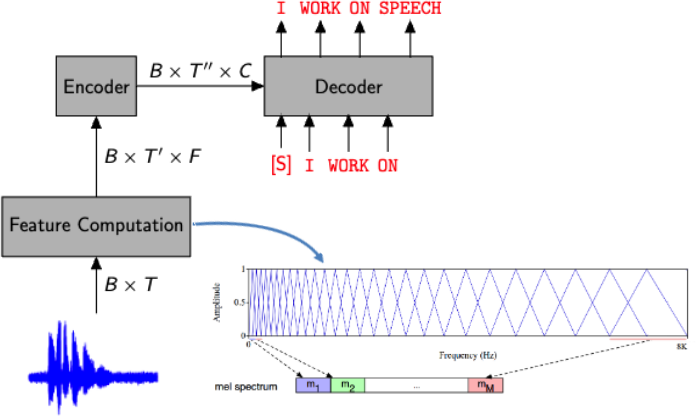
\includegraphics[width=0.5\linewidth]{./img/asp_arch.png}
            \end{figure}
        \end{example}

    \item[Speech enhancement]
        Clear the sound signal.

    \item[Speech separation]
        Separate the different sources in a sound signal (e.g., differentiate speakers).

    \item[Text-to-speech]
        Convert text into a sound signal.

        \begin{example}
            Use an encoder-decoder architecture. A text is processed as follows:
            \begin{enumerate}
                \item Use the encoder to embed the input text into a representation that encodes linguistic features (e.g., pronunciation, rhythm, \dots).
                \item Use the decoder to predict a mel-spectrogram.
                \item Use a neural vocoder to convert the mel-spectrogram into an audio waveform.
            \end{enumerate}

            \begin{figure}[H]
                \centering
                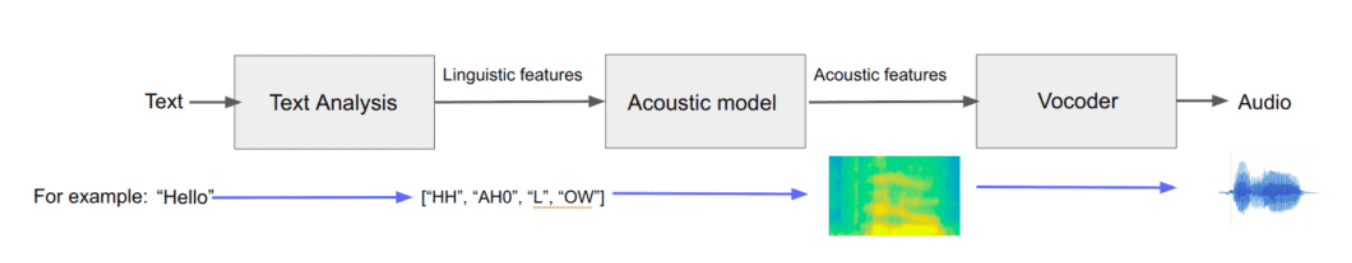
\includegraphics[width=0.9\linewidth]{./img/tts_arch.png}
            \end{figure}
        \end{example}

    \item[Speaker diarization]
        Determine the moment and the person who spoke.

    \item[Speech emotion recognition]
        Recognize emotions from the sound signal.

    \item[Neural network explanation]
        Use speech to explain another speech.
\end{description}



\section{Speech foundation models}


\begin{description}
    \item[Speech foundation model (SFM)] \marginnote{Speech foundation model (SFM)}
        Transformer-based model pre-trained on speech. A common architecture is composed of:
        \begin{descriptionlist}
            \item[Feature extractor] 
                Converts the waveform into a low-dimensional representation (e.g., by using convolutions).
            \item[Encoder] 
                Computes contextual embeddings from the sound features.
        \end{descriptionlist}

        \begin{remark}
            SFM takes as input raw waveforms and are more robust in dealing with speech variability due to diverse speakers, environment, noise, \dots
        \end{remark}

        \begin{remark}
            A SFM can be either fine-tuned for a specific task or used as a feature extractor for other models.
        \end{remark}

    \item[Multimodal model] \marginnote{Multimodal model}
        Model able to handle multiple modalities (e.g., speech and text). 

        The main considerations to take into account when working with multimodal models are:
        \begin{descriptionlist}
            \item[Representation] 
                Decide how to encode different modalities into the same embedding space.
            \item[Fusion]
                Combine information from different modalities.
            \item[Alignment]
                Link corresponding elements (e.g., in time or by meaning) across different modalities.
            \item[Translation]
                Map information from one modality to another.
            \item[Co-learning]
                Leverage shared information between modalities for training.
        \end{descriptionlist}
\end{description}